%-------------------------------------------
\begin{frame}{\raisebox{-1.5ex}{
\includegraphics[height=1cm]{shared/logo-github.png}} "Who” ?}
%-------------------------------------------
\begin{block}{Quizz}
\begin{enumerate}
    \item public institute (governmental)?
    \item semi-public institute?
    \item not-for-profit organisation?
    \item private company?
\end{enumerate}
\end{block}
\begin{block}{Response}
See \url{https://github.com/about}: Careers' paragraph, you'll see a "company" word
\end{block}
\end{frame}
%-------------------------------------------
\begin{frame}{GitLab, a \raisebox{-1.5ex}{
\includegraphics[height=1cm]{shared/logo-github.png}} alternative?}
%-------------------------------------------
\begin{center}

\includegraphics[height=5cm]{05_history/Images/FAIR_gitlab_company.png}
\end{center}
\end{frame}
%-------------------------------------------
\begin{frame}{\raisebox{-1.5ex}{
\includegraphics[height=1cm]{shared/logo-github.png}} “What” ?}
%-------------------------------------------
\begin{block}{Quizz}
\begin{enumerate}
    \item social network?
    \item desktop application?
    \item tool to create websites?
    \item stable repository to publish any file?
\end{enumerate}
\end{block}
\end{frame}
%-------------------------------------------
\begin{frame}[t]{
\includegraphics[height=1cm]{shared/logo-github.png}}
%-------------------------------------------
\begin{columns}[T]
\column{0.46\textwidth}
\begin{block}{a social network 
\includegraphics[height=0.3cm]{05_history/Images/FAIR_yes.png}}
\begin{center}
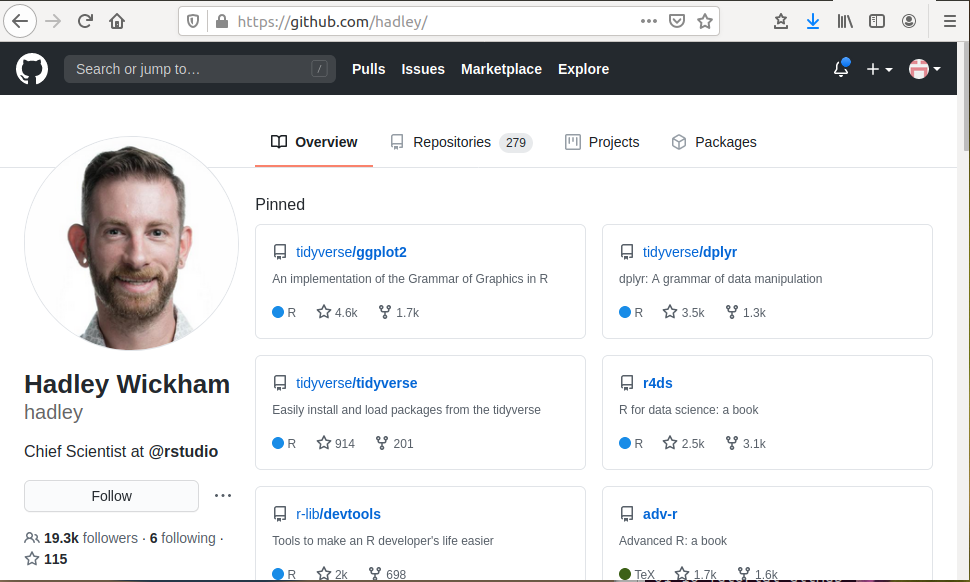
\includegraphics[height=2.6cm]{05_history/Images/FAIR_github_exSocialNet.png}
\end{center}
\end{block}
\begin{block}{a desktop application 
\includegraphics[height=0.3cm]{05_history/Images/FAIR_yes.png}}
\begin{center}
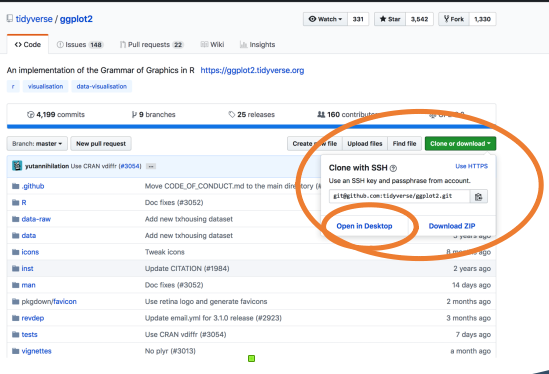
\includegraphics[height=2.6cm]{05_history/Images/FAIR_github_desktop_dl.png}
\end{center}
\end{block}
\column{0.46\textwidth}
\begin{block}{a tool to create websites 
\includegraphics[height=0.3cm]{05_history/Images/FAIR_yes.png}}
\begin{center}

\includegraphics[height=2cm]{05_history/Images/FAIR_github_pages.png}
\end{center}
\end{block}
\begin{block}{a stable repository ...}
\begin{center}
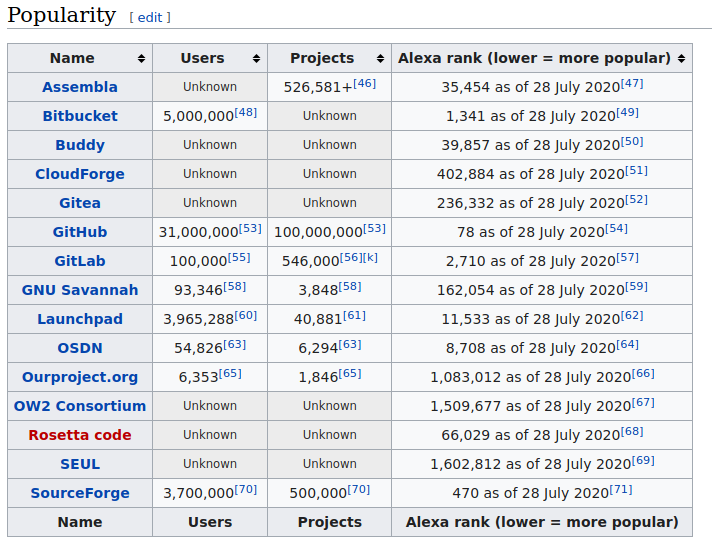
\includegraphics[height=2.4cm]{05_history/Images/FAIR_github_popularity.png}\\
{\tiny 
\href{https://en.wikipedia.org/wiki/\\
Comparison_of_source-code-hosting_facilities}{\textcolor{blue}{\underline{en.wikipedia}}}, comparison of source-code-hosting facilities
}
\end{center}
\end{block}
\end{columns}
\end{frame}
%-------------------------------------------
\begin{frame}{
\includegraphics[height=1cm]{shared/logo-github.png}}
%-------------------------------------------
\begin{columns}
\column{0.46\textwidth}
\begin{block}{a social network 
\includegraphics[height=0.3cm]{05_history/Images/FAIR_yes.png}}
\begin{center}
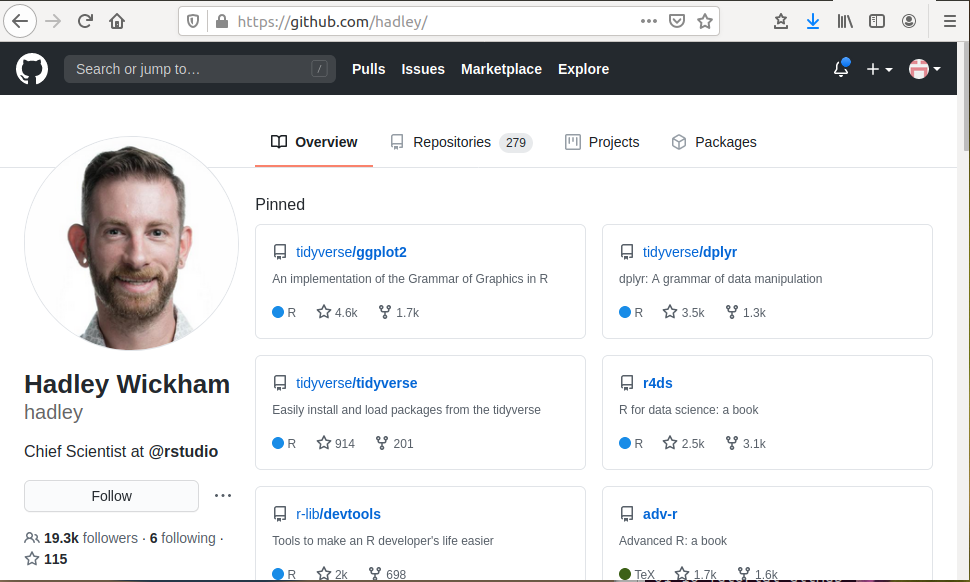
\includegraphics[height=2.6cm]{05_history/Images/FAIR_github_exSocialNet.png}
\end{center}
\end{block}
\begin{block}{a desktop application 
\includegraphics[height=0.3cm]{05_history/Images/FAIR_yes.png}}
\begin{center}
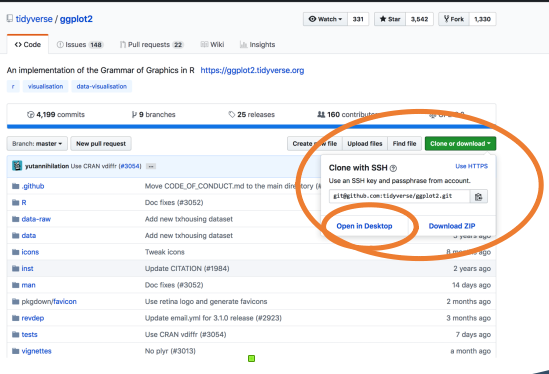
\includegraphics[height=2.6cm]{05_history/Images/FAIR_github_desktop_dl.png}
\end{center}
\end{block}
\column{0.46\textwidth}
\begin{block}{a tool to create websites 
\includegraphics[height=0.3cm]{05_history/Images/FAIR_yes.png}}
\begin{center}

\includegraphics[height=2cm]{05_history/Images/FAIR_github_pages.png}
\end{center}
\end{block}
\begin{block}{... to publish any file 
\includegraphics[height=0.3cm]{05_history/Images/FAIR_yes.png} 
\includegraphics[height=0.3cm]{05_history/Images/FAIR_no.png}}
Files for which git can calculate the difference between versions.
Usually txt files of reasonable size:\\
- R script: 
\includegraphics[height=0.3cm]{05_history/Images/FAIR_yes.png}\\
- Python script: 
\includegraphics[height=0.3cm]{05_history/Images/FAIR_yes.png}\\
- pdf file: 
\includegraphics[height=0.3cm]{05_history/Images/FAIR_no.png}\\
- fastq file: 
\includegraphics[height=0.3cm]{05_history/Images/FAIR_no.png}
\end{block}
\end{columns}
\end{frame}
%-------------------------------------------
\begin{frame}[containsverbatim]
\frametitle{\raisebox{-1.5ex}{
\includegraphics[height=1cm]{shared/logo-github.png}} main usage: sharing code with others}
%-------------------------------------------
\begin{block}{GitHub:}
\begin{itemize}
    \item so used that Microsoft was interested in it (\href{https://blogs.microsoft.com/blog/2018/06/04/microsoft-github-empowering-developers/}{\textcolor{blue}{\underline{bought}}} in june 2018)
    \item web-based: graphical interface + many more features than git
    \item git-based: git concepts and commands are retained
    \item commands for "sharing": \verb|git push origin master| (local to remote) and \verb|git pull origin master| (remote to local):
\end{itemize}
\begin{center}
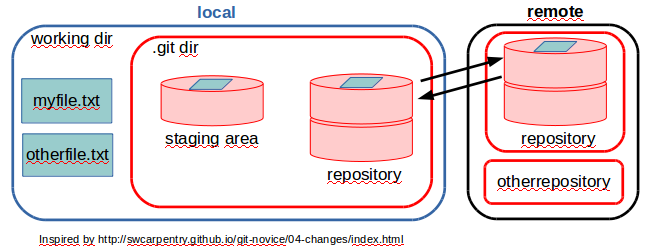
\includegraphics[height=3.5cm]{05_history/Images/FAIR_git_pushpull.png}
\end{center}
\end{block}
\end{frame}
%-------------------------------------------
\begin{frame}{
\includegraphics[height=1cm]{shared/logo-github.png} }
%-------------------------------------------
\begin{block}{Concepts, objects}
\begin{itemize}
    \item user: your account on GitHub (unlimited for academics)
    \item organization: account for one or more user (e.g., swcarpentry)
    \item local GitHub: copies of GitHub files located your computer
    \item remote GitHub: your GitHub files located on \href{https://github.com}{\textcolor{blue}{\underline{https://github.com}}}
    \item fork: a copy of a GitHub repository to your own GitHub account
    \item push: send changes on the working repository to your remote GitHub repository
    \item pull: copy changes on the remote GitHub repository to your local GitHub repository (useful when multiple people make changes)
    \item pull request: propose your changes to the initial forked GitHub repository. Also a place to compare and discuss the differences introduced on a branch with reviews, comments, integrated tests, etc
\end{itemize}
\end{block}
\end{frame}
%-------------------------------------------
\begin{frame}{\raisebox{-1.5ex}{
\includegraphics[height=1cm]{shared/logo-github.png}} Copy a project}
%-------------------------------------------
\begin{block}{Clone \textit{vs.} Fork?}
\begin{itemize}
    \item clone is git, fork is github
    \item all 2 copy a .git repository: clone copy it in your local machine, fork in your github account (do a clone)
    \item good practice: work (change files) in the local copy, not in the github copy (only for minor changes)
    \item to share your changes with the original repository, need a fork (by the way of a pull request)
\end{itemize}
\end{block}
See \href{https://opensource.com/article/17/12/fork-clone-difference}{\textcolor{blue}{\underline{here}}} an historical point of view of those 2 words.
\end{frame}
%-------------------------------------------
\begin{frame}{\raisebox{-1.5ex}{
\includegraphics[height=1cm]{shared/logo-github.png}} Copy a project}
%-------------------------------------------
\begin{block}{Recommended flow to collaborate}
\begin{columns}
\begin{column}{0.46\textwidth}
\begin{center}
    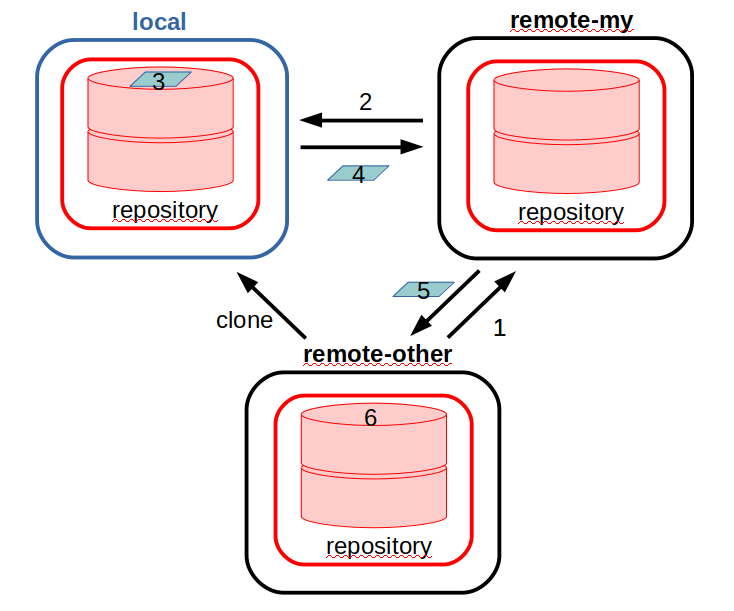
\includegraphics[height=5cm]{05_history/Images/FAIR_githubWFmaj.png}\\
    \small{(direct clone from github don't allow to collaborate)}
\end{center}
\end{column}
\begin{column}{0.5\textwidth}
\begin{itemize}
    \item 1: fork a repository of interest in your github account 
    \item 2: clone from your github account to your local place
    \item 3: make change (branch, add, commit, merge)
    \item 4: push change to your github account
    \item 5: pull request to propose your change to the initial project
    \item 6: wait (discuss) for integrating your change or not
\end{itemize}
\end{column}
\end{columns}
\end{block}
\end{frame}
%-------------------------------------------
%\begin{frame}{GitHub development cycle}
%-------------------------------------------
%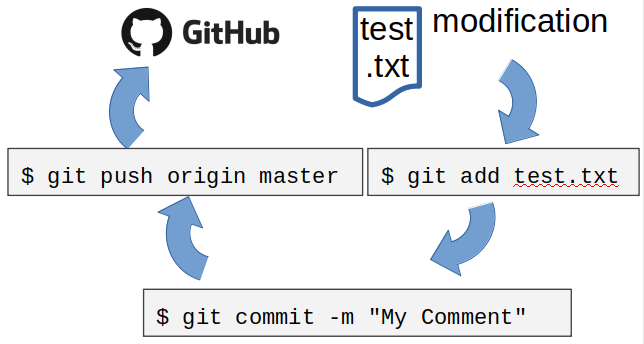
\includegraphics[height=5cm]{05_history/Images/FAIR_github_devCycle.png}
%\end{frame}